\documentclass[a4paper,14pt]{extarticle}
\usepackage{../../tex-shared/no-title-layout}

\begin{document}
\section{СЕРВЕРНОЕ ПРИЛОЖЕНИЕ НА ASP.NET CORE}
\subsection{Создание проекта и предназначение его классов}

Создадим проект ASP.NET Core с использованием пустого шаблона:

\begin{lstlisting}
md Practice
cd .\Practice
dotnet new sln --name PracticeTestApp
md PracticeTestApp
cd .\PracticeTestApp\
dotnet new web
cd ..
dotnet sln add .\PracticeTestApp\PracticeTestApp.csproj
\end{lstlisting}

Получим базовую структуру приложения, которое уже можно запустить (рисунок \ref{fig:project-structure}):

\begin{figure}[H]
    \centering
    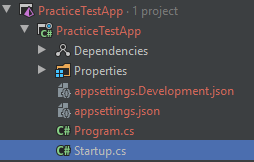
\includegraphics[width=.6\linewidth]{project-structure}
    \caption{Структура проекта}
    \label{fig:project-structure}
\end{figure}

На рисунке \ref{fig:project-structure} видно, что, помимо файлов непосредственно
проекта, проект содержит классы \code{Startup.cs} и \code{Program.cs}. Разберем
содержимое и предназначение этих файлов:

\subsubsection{\code{Program.cs}}

Содержимое \code{Program.cs} после создания пустого проекта:

\begin{lstlisting}
public class Program {
    public static void Main(string[] args) {
        CreateHostBuilder(args).Build().Run();
    }

    public static IHostBuilder CreateHostBuilder(string[] args) =>
        Host.CreateDefaultBuilder(args)
            .ConfigureWebHostDefaults(webBuilder => { webBuilder.UseStartup<Startup>(); });
}
\end{lstlisting}

Все приложения .NET Core по соглашению должны иметь точку входа в виде метода
\code{Main} класса \code{Program}. В этом месте в приложении ASP.NET Core
создается \code{Host} - абстракция для инкапсуляции всех ресурсов приложения:

\begin{itemize}
    \item реализация HTTP сервера;
    \item конфигурация сервера;
    \item компоненты конвейера;
    \item сервисы инверсии зависимостей (DI);
    \item логирование.
\end{itemize}

Есть два вида хостов: \code{.NET Generic Host}, \code{ASP.NET Core Web Host}.

Рекомендуется использовать \code{.NET Generic Host}, \code{ASP.NET Core Web
Host} нужет для обратной совместимости с прошлыми версиями ASP.NET Core.

Создание хоста происходит с вызовом метода \code{CreateDefaultBuilder}, который
устанавливает для хоста набор значений по умолчанию:

\begin{itemize}
    \item использование \code{Kestrel} в качестве веб сервера;
    \item использование \code{appsettings.json} и
          \code{appsettings.\\{EnvironmentName}.json}
          в качестве проводников конфигурации;
    \item перенаправление вывода логирования в консоль и инструменты отладки.
\end{itemize}

Кроме того, при создании хоста указывается, какой класс использовать в качестве
\code{Startup}.

\subsubsection{\code{Startup.cs}}

Содержимое класса \code{Startup.cs} после создание проекта:

\begin{lstlisting}
public class Startup {
    public void ConfigureServices(IServiceCollection services) { }

    public void Configure(IApplicationBuilder app, IWebHostEnvironment env) {
        if (env.IsDevelopment()) {
            app.UseDeveloperExceptionPage();
        }

        app.UseRouting();
        app.UseEndpoints(endpoints => {
            endpoints.MapGet("/", async context => {
                await context.Response.WriteAsync("Hello World!");
            });
        });
    }
}
\end{lstlisting}

\code{Startup.cs} - класс, в котором:

\begin{itemize}
    \item настраиваются сервисы, используемые приложением (метод\\
          \code{ConfigureServices});
    \item настраивается конвейер обработки HTTP запросов как список
          промежуточных компонентов middleware (метод Configure).
\end{itemize}

В базовом варианте класс просто задает ответ на все GET-запросы как строку
\enquote{Hello World!}.

\subsection{Настройка сервера под MVC архитектуру}
\subsubsection{Настройка роутинга}

Изначально ASP.NET Core проектировался под архитектуру MVC, поэтому настройка
включит в себя только включение MVC и настройка роутинга на контроллеры
MVC. Делается это следующим образом:

\begin{lstlisting}
public void ConfigureServices(IServiceCollection services) {
    services.AddMvc();
}
...
app.UseEndpoints(endpoints => {
    endpoints.MapControllerRoute(name: "default",
                                 pattern: "{controller=Home}/{action=Index}/{id?}");
});
\end{lstlisting}

Теперь запросы будут мэппиться на экшены и контроллеры с соответствующими
именами. Для обработки запросов нужно создать контроллер и экшен. Экшен -- любой
публичный метод контроллера, обычно возвращающий IActionResult. Url для
контроллера можно задать атрибутом.

\begin{lstlisting}
[Route("home")] 
public class HomeController : Controller {
    public IActionResult Index() => Ok();
}
\end{lstlisting}

Но лучше соблюдать соглашения по расположению контроллеров. В этом случае,
достаточно разместить контроллер в папке \code{Controllers}:

\begin{lstlisting}
namespace PracticeTestApp.Controllers { 
    public class HomeController : Controller {
        public IActionResult Index() => Ok();
    }
}
\end{lstlisting}

В обоих случаях запрос /Home/Index обработается экшеном \code{Index} класса
\code{HomeController}.

\subsubsection{Возвращение HTML документа}

Для того, чтобы вернуть HTML (в терминах MVC - View), нужно из экшена вернуть
\code{ViewResult}:

\code{public IActionResult Index() => View();}

Для view можно задавать имя, но, как и в случае с контроллерами, можно его
создать в папке Views в папке с именем соответствующего контроллера с именем
соответствующего экшена. View представляет из себя \code{.cshtml} документ,
использующий синтаксис \code{Razor}. \code{Razor} позволяет прокидывать из
контроллера во view необходимые данные и использовать их во view с помощью
синтаксиса C\#.

Создадим view, соответствующую экшену \code{Index}:

\begin{lstlisting}
//HomeController.cs:
public class HomeController : Controller {
    public IActionResult Index() {
        return View(new IndexViewModel("Hello, World!"));
    }
}

//IndexViewModel.cs:
public class IndexViewModel {
    public IndexViewModel(string message) {
        Message = message;
    }
    public string Message { get; }
}

//Views\Home\Index.cshtml:
@model PracticeTestApp.ViewModels.Home.IndexViewModel
<!DOCTYPE html>
<html>
    <head>
        <title>Test</title>
    </head>
    <body>
        <h1>@Model.Message</h1>
    </body>
</html>
\end{lstlisting}

При запуске приложени получим следующее (рисунок \ref{fig:view-testing}):

\begin{figure}[H]
    \centering
    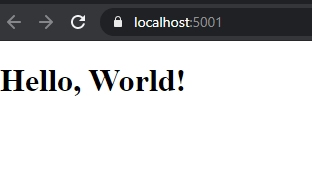
\includegraphics[width=.6\linewidth]{view-testing}
    \caption{Веб-страница, возвращенная сервером}
    \label{fig:view-testing}
\end{figure}

Для того, чтобы получить параметры из query string при GET запросе, достаточно
указать имена соответствующих параметров в экшене:

\code{public IActionResult Index(int id, string message)}

\subsubsection{Создание экшенов для других типов запросов}
Для обработки запросов, отличных от GET, достаточно задать атрибут
соответствующего запроса на экшене:

\begin{lstlisting}
public class HomeController : Controller {
    public IActionResult Index(int id, string message) {
        return View(new IndexViewModel("Hello, World!"));
    }

    [HttpPost]
    public IActionResult PostAction() => Ok();

    [HttpPut]
    public IActionResult PutAction() => Ok();

    [HttpDelete]
    public IActionResult DeleteAction() => Ok();
}
\end{lstlisting}

\subsection{Создание API-контроллеров}

API-контроллеры помечаются атрибутом \code{[ApiController]}. Желательно\\указывать
отдельный путь для API запросов. Пример:

\begin{lstlisting}
//DataController.cs
[ApiController]
[Route("api/[controller]")]
public class DataController : ControllerBase {
    [HttpGet]
    public ActionResult<string[]> Get() {
        var strings = new[] {
            "1", "2", "3", "4", "5"
        };
        return strings;
    }

    [HttpPost]
    public ActionResult<Product[]> Post() {
        var products = new[] {
            new Product(1, name: "First", type: "Utilities"),
            new Product(2, name: "Second", type: "Sports"),
            new Product(3, "Third", "Other")
        };
        return products;
    }
}

//Product.cs
public class Product {
    public Product(long id, string name, string type) {
        Id = id;
        Name = name;
        Type = type;
    }

    public long Id { get; }

    public string Name { get; }

    public string Type { get; }
}
\end{lstlisting}

Теперь, для того, чтобы обратиться к API-контроллеру, достаточно послать GET или
POST запросы на адрес \textbackslash api \textbackslash data (рисунки
\ref{fig:api-get} и \ref{fig:api-post}). Для отправки запросов используется
Postman.

\begin{figure}[H]
    \centering
    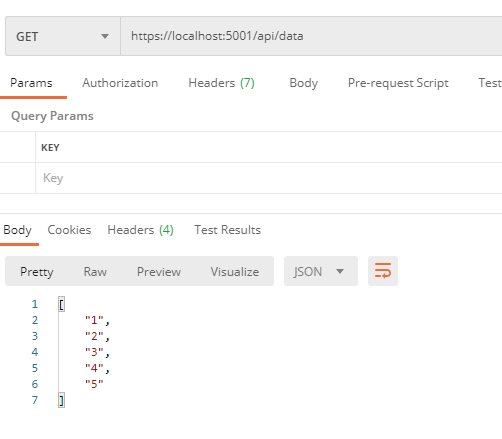
\includegraphics[width=.6\linewidth]{api-get}
    \caption{Получение результата GET-запроса}
    \label{fig:api-get}
\end{figure}

\begin{figure}[H]
    \centering
    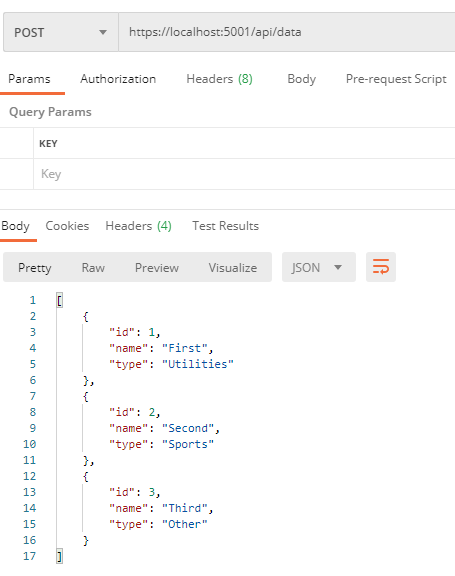
\includegraphics[width=.6\linewidth]{api-post}
    \caption{Получение результата POST-запроса}
    \label{fig:api-post}
\end{figure}

\subsection{Создание фильтров}

Фильтры в ASP.NET Core позволяют запускать код до или после определенных этапов
конвейера обработки запросов. Встроенные возможности аутентификации,
авторизации, кеширования ответов ASP.NET реализованы с помощью фильтров.

Очередь фильтров наступает после того, как фреймворк выбирает экшен, который
необходимо выполнить. Существуют следующие виды фильтров:

\begin{enumerate}
    \item Фильтры авторизации. Они запускаются первыми чтобы определить,
          авторизован ли пользователь для выполнения данного экшена. Они способны
          прерывать выполнение конвейера в том случае, если полььзователь не
          авторизован.
    \item Фильтры ресурсов. Следующие по вложенности фильтры.\\
          \code{OnResourceExecuting} выполняется перед всем остальным
          конвейером,\\\code{OnResourceExecuted} - после.
    \item Экшен фильтры. Выполняются непосредственно до и после вызова экшена.
          способны изменять параметры, передаваемые в экшены и мутировать
          результат выполнения экшена.
    \item Фильтры исключений. Используются для создания общего подхода к обработке
          необработанных исключений перед тем, как сформировать тело ответа.
    \item Фильтры результатов. Используются для запуска кода непосредственно после
          выполнения экшенов для мутирования результатов. Полезны для задания логики
          обработки View.
\end{enumerate}

Создадим фильтр и включим его в конвейер обработки запросов:

\begin{lstlisting}
//InvalidModelStateFilter.cs
public class InvalidModelStateFilter : IActionFilter {
    public void OnActionExecuted(ActionExecutedContext context) { }

    public void OnActionExecuting(ActionExecutingContext context) {
        if (!context.ModelState.IsValid) {
            context.Result = new BadRequestObjectResult(context.ModelState);
        }
    }
}

//Startup.cs
services.AddMvc(options => options.Filters.Add(typeof(InvalidModelStateFilter)));
\end{lstlisting}

Флаг ModelState отвечает за успешность привязки входящих параметров к объектам.
Приведенным выше способом можно валидировать входящие объекты, например, следующий
экшен принимает объект:

\code{public IActionResult IndexForProduct(Product product) => Ok();}

Обратимся к нему следующим образом:

\code{/Home/IndexForProduct?Id=15\&Name=hello\&type=sometype}

Получим ответ 200.

Обратимся, задав параметру Id невалидное значение:

\code{/Home/IndexForProduct?Id=asd\&Name=hello\&type=sometype}

Получим следующий ответ (рисунок \ref{fig:binder-error}):

\begin{figure}[H]
    \centering
    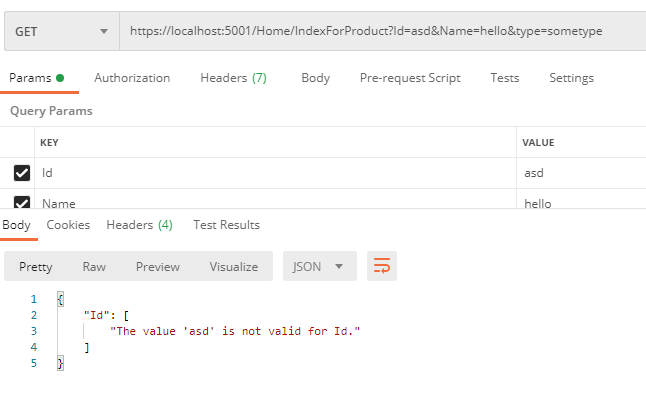
\includegraphics[width=.6\linewidth]{binder-error}
    \caption{Полученная ошибка при выполнении отправке невалидных данных}
    \label{fig:binder-error}
\end{figure}

\end{document}